\documentclass{article}
\usepackage{graphicx} % Required for inserting images
\usepackage{float} % Required for images
\usepackage{amsmath}

\begin{document}

\subsection{Análisis del circuito RL}
El error del cálculo de $\tau$ es menor al 1\%. Este error resulta pequeño pues se han tenido en cuenta la no idealidad de los instrumentos utilizados en las simulaciones.Además, este error se encuentra dentro del error de medición de los instrumentos utilizados. Sin embargo, a la hora de realizar los cálculos se ha tenido en cuenta como el valor final de $V_{RF}$  2,40V cuando en la experiencia se midieron 2,42V. 

El valor medido de la tensión de $R_F$ es menos de 1\% menor que el valor calculado. Este error resulta coherente con el error de los instrumentos utilizados. En este caso, no resulta lógico que el valor de la tensión medida sea menor que el calculado pues el $\tau$ medido resultó ser mayor al esperado. Consideramos que este efecto es causa de haber calculado $\tau$ con un pequeño error. 

Por último, el resultado que presenta una mayor diferencia con el calculado de esta parte de la experiencia es el tiempo en el que $R_F$ llega al 95\% de su valor final. Este error es aproximadamente del 5\% siendo el valor medido menor al calculado. Podemos atribuirle este error a la acumulación de errores anteriores en el cálculo de $\tau$ y también por trabajar con una precisión mayor a la que el instrumento trabaja.


De estos últimos resultados se puede concluir que el circuito tardará menos tiempo que el calculado en llegar al estado estacionario y que tendrá una tensión levente mayor al esperado. A nivel general, los resultados son coherentes con los calculados.

\subsection{Análisis del sistema RLC en serie}
Se puede observar en la experiencia que, al variar la resistencia $R_V$, cambia la respuesta transitoria. Partiendo desde el valor mínimo de $R_V$, se observó el mayor sobrepico de toda la experiencia y la oscilación más pronunciada de la respuesta transitoria antes de estabilizarse. En este caso, se estaba observando un sistema subamortiguado.

Al aumentar la resistencia paulatinamente, se observó la disminución de estos valores hasta llegar al punto en el que no había más sobrepico ni oscilaciones, correspondiente a un sistema con amortiguamiento crítico. Luego de ese punto, al seguir aumentando la resistencia hasta el máximo, se notó que el sistema tardaba cada vez más en alcanzar el equilibrio, lo que indica que se encontraba en un régimen sobreamortiguado.


\subsubsection{Sistema en amortiguamiento crítico}
Se buscó encontrar experimentalmente el valor de la resistencia para el cual el tiempo de llegada al equilibrio fuera mínimo. Sin embargo, en la práctica resulta complicado variar manualmente la resistencia hasta encontrar el punto exacto en el cual el sistema se encuentra críticamente amortiguado. Esto se debe a que es muy difícil distinguir entre un sistema críticamente amortiguado, un sistema sobreamortiguado con una leve diferencia entre $\omega_0$ y $\alpha$, y un sistema subamortiguado con una frecuencia de oscilación muy baja.

Se varió la resistencia de forma tal que, en el osciloscopio, se observara una curva con una pendiente pronunciada y sin sobrepico visible, intentando acercarnos lo mas posible al valor de la resistencia en el que $W_0 = \alpha_0$. No obstante, esta observación no implica que se haya alcanzado el valor real que minimiza el tiempo de estabilización.

Consecuentemente, debido a las dificultades previamente mencionadas, al contrastar el valor calculado de la resistencia con el valor medido, el error resultante fue bastante grande, llegando aproximadamente al 10\%.

\subsubsection{Sistema sobreamortiguado}
El tiempo $\tau_1$ obtenido experimentalmente resulta ser un 6\% mayor que el valor teórico. Si bien este error no es significativamente alto, puede deberse a que no se está considerando con precisión la resistencia interna de la bobina, lo que incrementa la resistencia equivalente del circuito. Esta modificación en la dinámica del sistema genera un sistema real más sobreamortiguado que el considerado teóricamente, lo que explica el aumento en el tiempo necesario para alcanzar el $63\%$ del valor máximo de $v_C$ en la práctica.

Por otro lado, la tensión $V_C$ medida luego de un tiempo $5\tau_1$ resulta ser menos de un 1\% mayor que la estimada teóricamente. Este resultado no es necesariamente incoherente con el anterior, ya que la diferencia entre el valor esperado (4,96 V) y el medido (5 V) puede atribuirse a la resolución y precisión limitada de los instrumentos de medición.

A partir de estos resultados, se puede concluir que la aproximación de considerar $5\tau_1$ como el tiempo necesario para que el sistema alcance el estado estacionario es válida dentro del margen de error experimental.


\subsection{Sistema subamortiguado}
Al medir el tiempo que tarda la tensión en llegar al $95\%$ de su valor final por primera vez, se obtuvo una diferencia menor al $3,5\%$ respecto del resultado observado en LTspice. Luego, al medir la frecuencia de oscilación y compararla con la calculada analíticamente, se obtuvo una discrepancia menor al $2\%$. Estos errores son pequeños y pueden atribuirse a la precisión limitada de los instrumentos utilizados.

Sin embargo, las mediciones de $V_C$ correspondientes al sobrepico máximo resultaron ser un $12,2\%$ menores que las obtenidas en LTspice utilizando los datos indicados en el TP y la impedancia calculada en el circuito RL. Esta diferencia sugiere que el sistema real presenta un amortiguamiento mayor que el considerado en la simulación.

Una posible explicación es que el modelo utilizado no contempla todas las pérdidas presentes en el inductor real. Entre ellas podrían encontrarse la resistencia interna de la bobina y, en caso de que el núcleo magnético tenga un comportamiento no ideal, pérdidas asociadas a fenómenos como la histéresis. La histéresis implica que la respuesta magnética del material depende de los estados previos de magnetización, lo que produce disipación de energía y reduce el sobrepico observado experimentalmente.

Si bien un mayor amortiguamiento reduce la frecuencia amortiguada $\omega_d$ y, en consecuencia, debería aumentar el tiempo de sobrepico $t_{so} = \pi/\omega_d$, experimentalmente se obtuvo un valor $10\%$ menor. Esto sugiere que la diferencia no se debe a que la medición experimental del tiempo de sobrepico presenta una incertidumbre significativa, ya que el pico no se encuentra perfectamente definido en la señal observada. La determinación del instante de máximo se realizó mediante cursores sobre el osciloscopio, lo que introduce un error asociado a la resolución del instrumento. Asimismo, el trigger no siempre se encontraba perfectamente ajustado, y el instante inicial del escalón puede no coincidir exactamente con el asumido, lo que impacta directamente en la medición del tiempo. 

Al estimar alfa como depende del $V_C$ del sobrepico y del $t_{so}$ se obtuvo una diferencia del $60\%$ respecto del calculado. Este mismo error se arrastra al calcular el tiempo $\frac{5}{\alpha}$. Luego al calcular la resistencia equivalente del circuito a partir del $\alpha$ estimado se obtuvo que el valor de la resistencia en serie del inductor debe ser aproximadamente 167 veces mas grande. Estos resultados concuerdan con el analisis anterior ya que implican que el circuito es mas resistivo que el esperado.

\subsection{Inductor con resistencia en paralelo; ítem g}
Al simular el mismo circuito modelando las pérdidas del inductor mediante una resistencia en paralelo, se observó que, cuanto mayor era el valor de $R_P$, más similar resultaba la respuesta a la de un circuito RLC ideal. Esto se debe a que, al aumentar $R_P$, la corriente que circula por la resistencia disminuye y, en consecuencia, la potencia disipada en dicha rama es menor.

En cambio, al tomar valores más pequeños de $R_P$, una mayor fracción de la corriente circula por la rama resistiva en paralelo, lo que incrementa las pérdidas del sistema y atenúa el efecto inductivo ideal. Como consecuencia, la respuesta transitoria presenta un mayor amortiguamiento y una menor oscilación.

La resistencia en paralelo que debería tener el modelo del inductor para reproducir la resistencia equivalente calculada se obtiene a partir de la equivalencia serie-paralelo:

\[
R_P=\frac{R_s^2+(\omega L)^2}{R_s}
\]

donde

\[
R_s = 2\alpha L - R_F - R_V - R_S
\]

Por lo tanto,

\[
R_P=\frac{(2\alpha L-R_F-R_V-R_S)^2+(\omega L)^2}{2\alpha L-R_F-R_V-R_S}
\]

Utilizando los valores experimentales obtenidos, se calculó un valor de $R_P \approx 2{,}5~\text{k}\Omega$.

\begin{figure}[H]
\centering
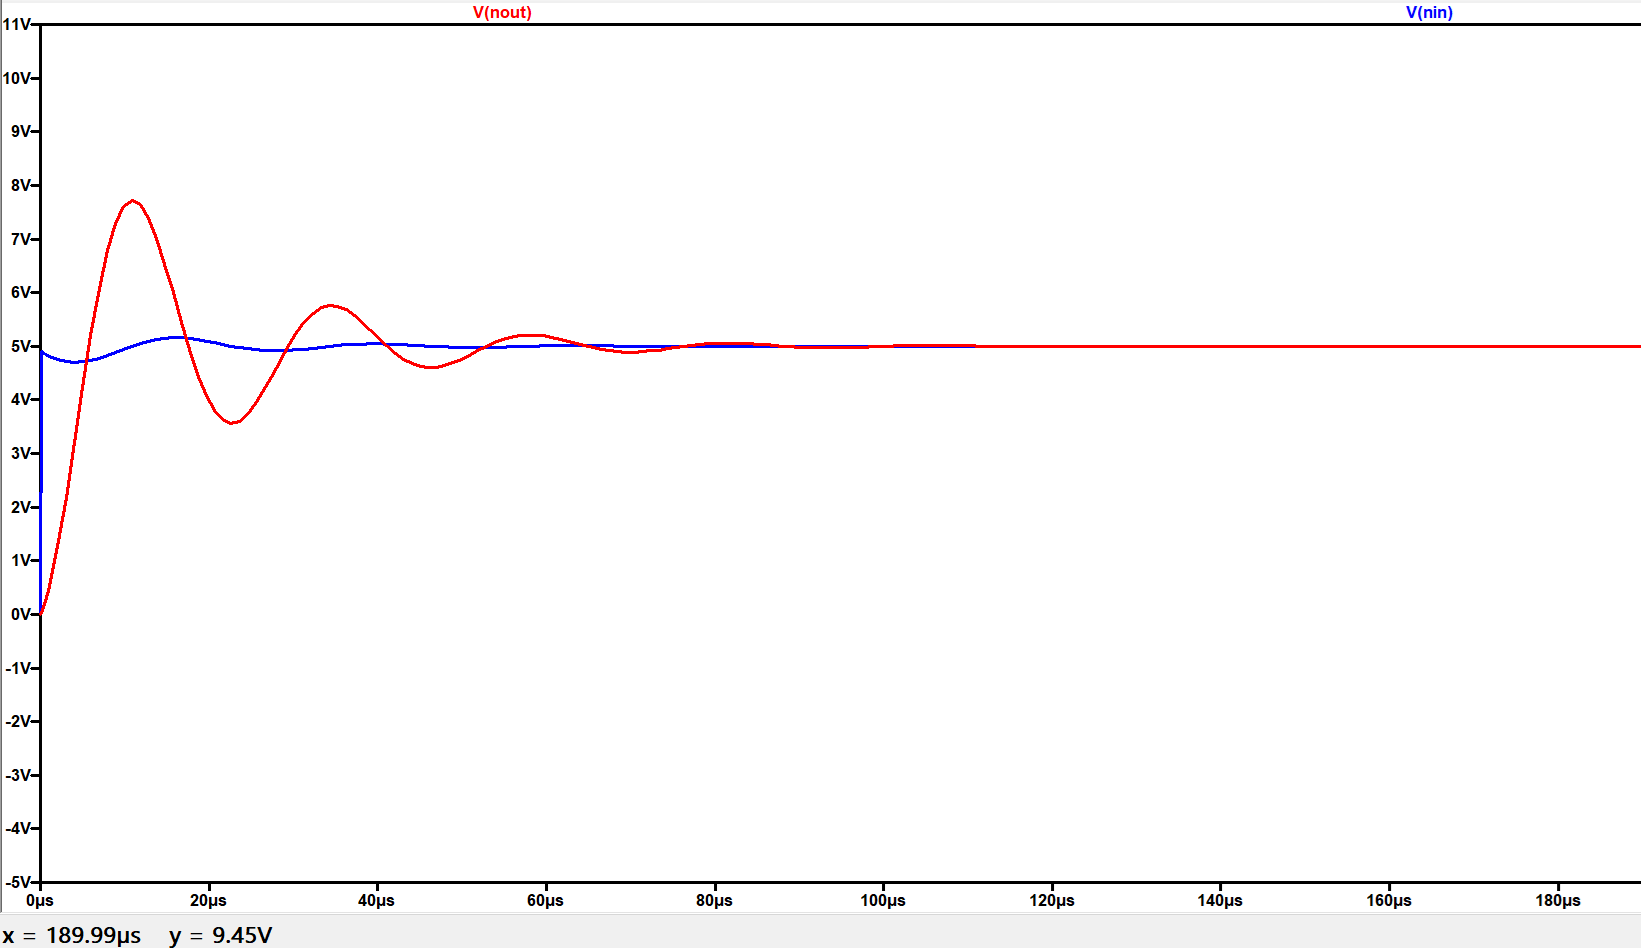
\includegraphics[width=0.6\textwidth]{simulacion_g_RP.png}
\caption{Grafico en el tiempo de la diferencia de potencial en la fuente ( V(nin) ) y en el capacitor ( V(nout))con $R_L$ en parlelo}
\label{fig:sim_g_RP} 
\end{figure}

\begin{figure}[H]
\centering
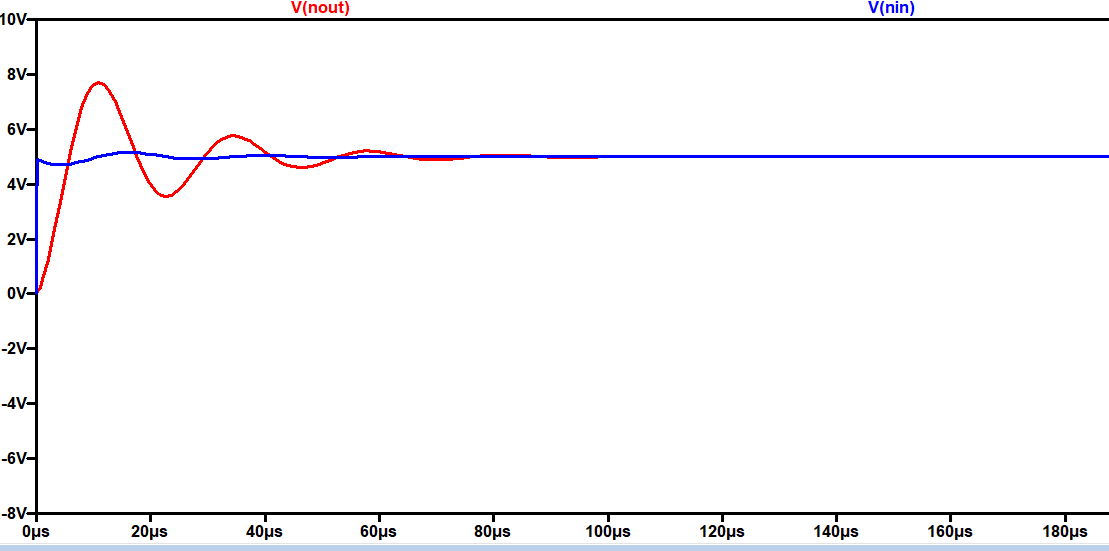
\includegraphics[width=0.6\textwidth]{sim_g_RS.png}
\caption{Grafico en el tiempo de la diferencia de potencial en la fuente ( V(nin) ) y en el capacitor ( V(nout)) con $R_L$ en serie}
\label{fig:sim_g_RS} 
\end{figure}

Al comparar la simulación utilizando un modelo de pérdidas en serie con aquella que emplea una resistencia en paralelo, se observa:

En ambos casos, la respuesta mantiene un comportamiento subamortiguado, con presencia de sobrepico y oscilaciones decrecientes. Sin embargo, al utilizar una resistencia en paralelo, se observa una ligera reducción en la amplitud de las oscilaciones y un decaimiento más pronunciado en los primeros ciclos, lo que indica una disipación de energía más efectiva en ese rango temporal.

Por otro lado, el modelo con resistencia en serie tiende a preservar mejor la forma global de la respuesta oscilatoria, manteniendo una relación más directa con el modelo teórico de un RLC serie ideal con pérdidas distribuidas uniformemente.

\end{document}
